% ======================================================================
%  Chapter: The Cartography of Physical Theories
%
%  Intended to be \input{} or \include{}'d from the book's master file.
%  Assumes the master preamble loads at least:
%    \usepackage{amsmath,amssymb}
%    \usepackage{tikz}
%  No bibliography file is required -- all historical results are
%  named in the text rather than cited by key, so the chapter compiles
%  standalone if wrapped in a minimal \documentclass{book} shell.
% ======================================================================

\chapter{The Cartography of Physical Theories}
\label{ch:cartography}

\section{The received view}
\label{sec:received-view}

Textbooks state, almost as a matter of course, that classical mechanics is recovered from special relativity in the limit $c\to\infty$, that it is recovered from quantum mechanics in the limit $\hbar\to 0$, that thermodynamics is recovered from statistical mechanics in the limit $N\to\infty$, and that geometrical optics is recovered from wave optics in the limit $\lambda\to 0$. In each case a single dimensionless parameter is identified ($v/c$, $\hbar/S$, $1/N$, $\lambda/L$), sent to zero, and the parent theory is said to degenerate, term by term, into the child theory.

The picture earns its keep computationally. Expanding the relativistic energy
\[
E=\frac{mc^2}{\sqrt{1-v^2/c^2}} \;\approx\; mc^2+\tfrac12 mv^2+\cdots
\]
does produce the Newtonian kinetic energy at leading order; substituting the WKB ansatz $\psi=e^{iS/\hbar}$ into the Schr\"odinger equation and expanding $S=S_0+\hbar S_1+\cdots$ does produce the Hamilton--Jacobi equation $\tfrac{1}{2m}(\nabla S_0)^2+V=E$ at leading order. These calculations are correct and indispensable. What is not correct is the stronger claim made on their behalf: that they exhibit classical mechanics as \emph{the} limit of the parent theory -- a single, structurally faithful degeneration of it, in the way a circle is the limit of a family of ellipses as the eccentricity goes to zero.

This chapter argues that ``limit'' is the wrong figure of speech for the general relation between physical theories, and that a better one is available: two theories stand to one another roughly as two maps of the same territory stand to one another. Only along one very particular axis -- resolution -- is ``limit'' even approximately the right word, and even there it can fail.

\section{Two kinds of trouble with \emph{the} limit}
\label{sec:trouble}

\subsection{Objects with no image}
\label{subsec:missing}

A limit, in the ordinary mathematical sense, is a map: it takes every object of the parent theory to some object of the child theory. But classical mechanics is full of objects that are not the image of anything in special relativity or in quantum mechanics, because they presuppose structure the parent theory does not have.

A perfectly rigid body is the standard example: it requires instantaneous transmission of stress, which special relativity forbids outright (no signal, and in particular no sound wave enforcing rigidity, can outrun $c$). The $c\to\infty$ ``limit'' does not approximate rigid bodies with increasingly good relativistic rigid bodies; it manufactures rigidity out of nothing, by removing the very constraint (finite $c$) that made rigidity impossible. Friction is a second example, of a different kind: the microscopic laws, classical, relativistic, or quantum, are time-reversal invariant, while friction is not. No amount of letting $\hbar\to 0$ inside a Hamiltonian, unitary, reversible quantum theory produces an irreversible force; irreversibility only appears once one coarse-grains over unobserved degrees of freedom, which is a different operation entirely (and, tellingly, one indexed by \emph{resolution}, the axis discussed in \S\ref{subsec:resolution} below, not by $\hbar$ or $c$). Nonholonomic constraints and bodies that change their own shape (treated at length in the chapter on strange things in classical mechanics) are a third example: they are formulated directly in terms of velocities and configuration space and simply have no counterpart to take a limit \emph{of} in a parent theory that knows nothing of extended, deformable, macroscopically constrained bodies.

In each case the moral is the same. The parent theory's limit is not a substructure of classical mechanics reached by forgetting detail; it is a proper subset of classical mechanics's subject matter, missing entire categories of object. A map that shows only roads cannot be said to reduce, in the limit of coarser printing, to a map that also shows roads, rivers, and political borders -- the borders were never on the road map to begin with.

\subsection{The limit itself is singular}
\label{subsec:singular}

Even restricted to the objects a parent theory \emph{does} know about, the limits in question are typically not smooth deformations but singular perturbations, in the technical sense familiar from Prandtl's boundary-layer theory: a small parameter multiplies the highest-order structure, so that setting it to zero changes the qualitative character of the description rather than merely its quantitative detail.

Three examples worth having on hand:

\begin{itemize}
\item \textbf{$c\to\infty$.} The passage from the Poincar\'e group to the Galilei group is an \.In\"on\"u--Wigner \emph{group contraction}: a well-defined but genuinely singular limit of the Lie algebra, in which the structure constants degenerate and a semisimple algebra (Poincar\'e) becomes a non-semisimple one (Galilei). Absolute simultaneity is not a slightly-better approximation to relativistic simultaneity; it is a different, degenerate causal structure that appears only exactly at $c=\infty$, nowhere before it.
\item \textbf{$\hbar\to0$.} The WKB approximation is uniformly good almost everywhere but fails at classical turning points and caustics, where classical trajectories focus or cross and the semiclassical wavefunction formally diverges; the correct local behavior there is given by Airy functions, not by the leading WKB term at smaller $\hbar$. Nor is there, even in principle, a single smooth ``quantization map'' running the other way: the Groenewold--van Hove theorem shows that no assignment of operators to phase-space functions can preserve the full Poisson-bracket algebra beyond quadratic polynomials, so the correspondence between the two pictures is an obstructed, not merely approximate, one.
\item \textbf{$N\to\infty$.} The free energy of a finite system is always an analytic function of temperature; genuine phase transitions -- the qualitative changes in macroscopic behavior that thermodynamics is largely \emph{about} -- appear only in the strict $N\to\infty$ limit, as the zeros of the partition function (Yang--Lee zeros) pinch onto the real axis. The interesting physics sits exactly at the singularity of the limit, not in its smooth bulk.
\end{itemize}

So the situation is worse than ``the limit is singular in some technical corner case.'' The singularities sit precisely where the physically interesting structure lives: at the light cone, at caustics, at phase transitions. A metaphor that treats these as removable blemishes on an otherwise faithful reduction gets the emphasis backwards.

\section{An analogy from cartography}
\label{sec:cartography}

Consider instead what it means for two maps to be maps ``of the same territory.'' Two maps can differ along at least four largely independent axes.

\begin{table}[h]
\centering
\renewcommand{\arraystretch}{1.3}
\begin{tabular}{p{2.2cm} p{5.6cm} p{5.6cm}}
\hline
\textbf{Axis} & \textbf{Cartography} & \textbf{Physics} \\
\hline
Theme & Political, physical, geological, and weather maps of the same region & Mechanics, thermodynamics, electromagnetism: different theories answering different questions about the same world \\
Projection & Mercator, Robinson, stereographic, gnomonic renderings of the same theme and extent & Lagrangian vs.\ Hamiltonian mechanics; Schr\"odinger vs.\ Heisenberg vs.\ path-integral pictures of quantum mechanics \\
Extent & Which portion of the globe is shown & Domain of validity: weak field vs.\ strong field, low speed vs.\ relativistic \\
Resolution & Scale, e.g.\ 1:1{,}000 vs.\ 1:1{,}000{,}000 & Coarse-graining: microscopic vs.\ macroscopic description \\
\hline
\end{tabular}
\caption{Four largely independent axes along which two representations of ``the same'' subject matter can differ.}
\label{tab:axes}
\end{table}

\subsection{Theme: what a theory is about}

A weather map and a political map of France are not related by any limiting procedure at all; neither is a coarsening or a refinement of the other, because they depict different things. Mechanics, thermodynamics, and electromagnetism stand in the same relation. Thermodynamics is not a low-resolution version of electromagnetism, nor a special case of it; it is a different thematic layer over the same territory, addressing questions (heat, entropy, equilibrium) that a purely mechanical or electromagnetic map does not attempt to answer. Demanding that thermodynamics arise as \emph{the} limit of electromagnetism would be as confused as demanding that a weather map arise as the limit of a political one.

\subsection{Projection: how a theory represents its subject}

Within a single theme, different projections of the same territory preserve different structure at the expense of other structure -- this is not a defect of cartography but a theorem about it. A conformal (angle-preserving) projection such as Mercator's cannot also be equal-area; an equal-area projection such as Albers's cannot also be conformal. Gauss's \emph{Theorema Egregium} makes the obstruction precise: a curved surface's intrinsic curvature cannot be flattened into the plane without distorting either lengths, angles, or areas -- there is no projection that gets everything right at once, only a menu of projections each suited to a different purpose (Mercator for navigation, Albers for area comparisons).

The different formalisms of a single physical theory are projections in exactly this sense, not distinct theories and not limits of one another. The Hamiltonian and Lagrangian formulations of classical mechanics carry the same content but make different structure legible: the Hamiltonian picture displays conserved quantities and symmetries transparently (as the book's chapter on the geometric versus coordinate formulations of mechanics discusses at length) while partially obscuring manifest covariance, which the Lagrangian picture, built from a scalar action, preserves more readily. The Schr\"odinger, Heisenberg, and path-integral pictures of quantum mechanics stand in the same relation to one another. None of this is a reduction; it is re-projection, and asking which picture is ``really'' the theory is as misguided as asking whether Greenland is ``really'' as big as Africa.

\subsection{Extent: domain of validity}

A street map of Paris does not contain Berlin, not because Berlin has been idealized away but because it was never in scope. In the same way, Newtonian gravitation's domain of validity (weak fields, low speeds) is a genuine subset of general relativity's, and special relativity's domain (no gravity at all) is neither contained in nor contains Newtonian gravity's domain -- the two extents overlap only partially. This axis is what turns the whole picture from a loose metaphor into something with real structure, developed formally in \S\ref{sec:atlas}.

\subsection{Resolution: the one genuine limit, and why even it can fail}
\label{subsec:resolution}

Only along the resolution axis is ``limit'' close to the right word. A 1:1{,}000{,}000 map genuinely can, in principle, be produced by coarse-graining a 1:1{,}000 map of the same theme, projection, and extent: this is a real limiting operation on one and the same representation, and it is the cartographic image of coarse-graining a microscopic statistical-mechanical description into a macroscopic thermodynamic one, or of a renormalization-group step integrating out short-distance degrees of freedom.

But even this limit routinely fails to be smooth. The length of a coastline, measured at increasing resolution, does not converge to a finite number: it grows without bound as the measuring scale shrinks, because coastlines are statistically self-similar over a wide range of scales (the coastline paradox, quantified by Richardson and Mandelbrot in terms of a fractal dimension greater than one). Only certain coarse features -- the shape of a bay, the overall outline of a continent -- stabilize under coarsening; the fine-grained quantity ``total length'' simply has no resolution-independent limit. The physical analogue is exact: the thermodynamic limit is singular precisely at a phase transition, where the system develops fluctuations at every length scale simultaneously (critical phenomena), and the renormalization-group flow sits at a fixed point at which ``resolution'' stops being a meaningful independent parameter at all. The one axis along which cartography licenses talk of a limit is also the one axis along which cartography itself warns that the limit can be singular.

\section{Formalizing the atlas}
\label{sec:atlas}

The extent axis (\S\ref{subsec:missing}, \S3.3) can be made precise using the same language already introduced for classical mechanics's relation to relativity and quantum theory: charts on a manifold.

Let $\mathcal{M}$ denote, informally, the totality of physical phenomena. A physical theory $T_i$ comes with a domain of applicability $U_i\subset\mathcal{M}$ -- ``speeds small compared to $c$,'' ``actions large compared to $\hbar$,'' ``system sizes for which surface effects are negligible'' -- and a chart
\[
\varphi_i : U_i \longrightarrow \mathcal{D}_i
\]
into some mathematical structure $\mathcal{D}_i$ (a phase space with a Hamiltonian flow, a Hilbert space with an algebra of operators, and so on). Where two domains overlap, $U_i\cap U_j\neq\varnothing$, consistency requires a transition map
\[
\varphi_j\circ\varphi_i^{-1} : \varphi_i(U_i\cap U_j)\longrightarrow \varphi_j(U_i\cap U_j)
\]
relating the two descriptions on the overlap. This is exactly what a correspondence principle is. Three consequences follow immediately, and each has already appeared above under another name:

\begin{itemize}
\item Transition maps are defined, and well-behaved, only on the overlap $U_i\cap U_j$ -- never globally. This is \S\ref{subsec:missing}'s point about objects with no image, restated: a rigid body simply is not in $U_{\text{SR}}\cap U_{\text{CM}}$.
\item Transition maps can be, and typically are, singular near the boundary of the overlap. This is \S\ref{subsec:singular}: the light cone at $v=c$, caustics at turning points, the pinching Yang--Lee zeros at a phase transition are all boundary phenomena of an overlap region, not interior ones.
\item A chart's domain need not contain, or be contained in, another's. General relativity's domain properly contains special relativity's and Newtonian gravity's; but the domain of continuum elasticity, with its rigid and frictional and shape-changing bodies, is not contained in the domain of single-particle relativistic quantum mechanics in any straightforward sense at all, because it requires additional statistical and macroscopic structure that single-particle theories do not supply.
\end{itemize}

\begin{figure}[h]
\centering
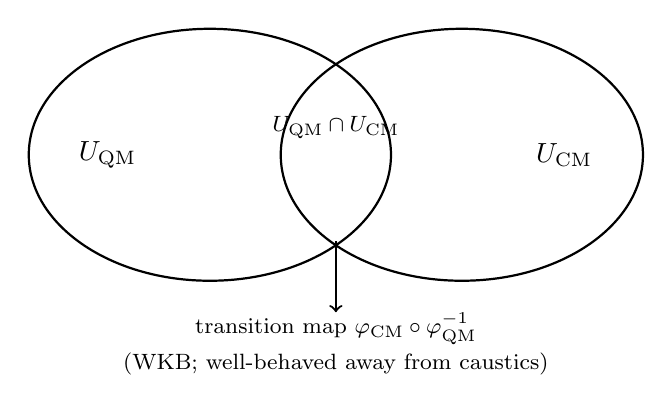
\begin{tikzpicture}[scale=1]
\draw[thick] (-1.6,0) ellipse (2.3 and 1.6);
\draw[thick] (1.6,0) ellipse (2.3 and 1.6);
\node at (-2.9,0) {$U_{\mathrm{QM}}$};
\node at (2.9,0) {$U_{\mathrm{CM}}$};
\node[align=center] at (0,0.35) {\footnotesize $U_{\mathrm{QM}}\cap U_{\mathrm{CM}}$};
\draw[->,thick] (0,-1.1) -- (0,-2.0);
\node[align=center] at (0,-2.4) {\footnotesize transition map $\varphi_{\mathrm{CM}}\circ\varphi_{\mathrm{QM}}^{-1}$\\[1pt]\footnotesize (WKB; well-behaved away from caustics)};
\end{tikzpicture}
\caption{Classical and quantum mechanics as two overlapping charts on the space of physical phenomena. Each is a complete, self-contained description on its own domain; the WKB correspondence is the transition map on their overlap, singular precisely at the caustics that sit near the overlap's boundary.}
\label{fig:atlas}
\end{figure}

A further, sharper parallel is available at the level of the projection axis (\S3.2). Gauss's \emph{Theorema Egregium} is a no-go theorem: no chart can flatten a curved surface while preserving all of length, angle, and area. The Groenewold--van Hove theorem is the same kind of no-go result one level up: no chart can carry the full Poisson-bracket structure of classical phase space onto the commutator structure of quantum operators. Both theorems say, in their own domains, that a perfect map does not exist -- only a family of imperfect maps, each preserving a different piece of structure, none of them dominant.

\section{Worked examples, revisited}
\label{sec:examples}

Bringing the pieces of \S\ref{sec:trouble}--\S\ref{sec:atlas} together against the four familiar reductions:

\begin{itemize}
\item \textbf{Classical / relativistic mechanics.} Overlap: low speed. Transition map: the Lorentz factor $\gamma$, well-behaved for $v\ll c$, singular exactly at $v=c$ -- the boundary of the overlap, and not coincidentally the edge of the light cone, whose disappearance under $c\to\infty$ is the \.In\"on\"u--Wigner contraction of \S\ref{subsec:singular}. Off-map object: the rigid body.
\item \textbf{Classical / quantum mechanics.} Overlap: large action compared to $\hbar$. Transition map: the WKB correspondence, singular at caustics and turning points, and in any case not invertible into a single consistent quantization scheme (Groenewold--van Hove). Off-map objects: nonholonomic constraints, shape-changing bodies, anything requiring an extended, classically-rigid or classically-constrained body rather than a point particle or field mode.
\item \textbf{Thermodynamics / statistical mechanics.} Overlap: large $N$, away from criticality. Transition map: the identification of thermodynamic potentials with appropriately averaged statistical quantities, singular precisely at phase transitions (Yang--Lee), where the resolution axis itself, as in the coastline paradox, ceases to yield a well-defined limiting quantity.
\item \textbf{Geometrical / wave optics.} Overlap: features large compared to $\lambda$. Transition map: the eikonal equation $|\nabla S|^2=n^2$, obtained from the Helmholtz equation at small $\lambda$, singular at caustics -- where, tellingly, real physical structure appears (a rainbow \emph{is} a caustic of sunlight in raindrops) rather than being merely an artifact of the approximation's failure.
\end{itemize}

In every case the same triple holds: a genuine overlap region, a transition map that is a good approximation deep inside it, and a singularity sitting at or near its edge that carries, rather than obscures, some of the theory's most characteristic physical content.

\section{Conclusion: the discipline of atlas-making}
\label{sec:conclusion}

If this is right, the project of relating physical theories to one another is better conceived as atlas-making than as limit-taking. An atlas does not aim at a single chart covering everything -- indeed, for a sphere no such chart exists without a coordinate singularity somewhere, a fact with the same flavor as the no-go theorems of \S\ref{sec:atlas}. It aims instead at a well-chosen cover, with transition maps that are explicit about where they are valid, honest about where they break down, and unapologetic about the fact that some regions require an altogether different theme, not merely a different resolution, to be represented at all.

This has the same shape as the real-world/ideal-world distinction developed elsewhere in this book. A cartographic error occurs when a feature of the map -- a projection's coordinate singularity at the pole, Greenland's inflated area under Mercator -- is mistaken for a feature of the territory. The corresponding physical error runs in both directions: treating the mathematical singularity of a correspondence limit as if it were merely a calculational inconvenience to be patched away, and, just as badly, dismissing a real emergent phenomenon that appears only at the singularity of a limit -- a phase transition, a caustic, the light cone itself -- as ``just'' an artifact of idealization. Both mistakes come from forgetting that a map, however good, is not the territory, and that the interesting places on any map are so often exactly where two of them stop agreeing.

